%%%%%%%%%%%%%%%%%%%%%%%%%%%%%%%%%%%%%%%%%%%%%%%%%%%%%%%%%%%
\section{Torque Control}
\label{sec:theory}
%%%%%%%%%%%%%%%%%%%%%%%%%%%%%%%%%%%%%%%%%%%%%%%%%%%%%%%%%%%
%\subsection{Controlling Torque}


The orientation of an object's major axis is important when a swarm is manipulating a non-symmetric object through narrow corridors. 
Orientation is controllable by applying torque to the object. 
To change the output torque $\tau$ in Eq.~\eqref{eq:torque}, we can choose the direction and magnitude of the force applied $F$, and the moment arm from the object's center of mass (COM) to the point of contact $r$.

\begin{equation}
\tau = F \times r\label{eq:torque}
\end{equation}
The swarm version of \eqref{eq:torque} is the summation of the forces contributed by individual robots.

\begin{align}
\tau_{total} &= \sum\limits_{i=1}^n \rho_i F_i \times (P_i - O )   \label{eq:swarmtorque}\\
F_{total} &= \sum\limits_{i=1}^n \rho_i F_i  \label{eq:swarmforce}
\end{align}

Here $F_i$ is the force that the $i$th robot applies.  If all robots are identical and the control input is uniform, the force is equivalent for every robot and $F_i = F_c$.
Not all robots are in contact with the object.  $\rho_i$ is an indicator variable: $\rho_i$ is 1 if the robot is in direct contact with the object or touching a chain of robots where at least one robot is in contact with the object. Otherwise $\rho_i = 0$.
The moment arm is the robot's position $P_i$ to the object's COM $O=[O_x,O_y]^{\top}$.

\section{Instantiation of torque from robot distribution}
Consider a swarm of robots with probability density $p(x)$. This section examines where to steer the mean of the probability distribution to maximize torque. We examine two problems. First, the torque applied to a rod of length 1 pivoted at 0 when $\theta = 0$ is:
\begin{equation}
\tau_{pivot} = \int_0^1 xp(x)\, dx
\end{equation}
Second, the torque applied to a free rod of length 2 from $[-1,0]$ to $[1,0]$, is:
\begin{equation}
\tau_{free} = \int_{-1}^1 xp(x)\, dx
\end{equation}
This section considers three canonical probability distributions: uniform, triangular, and normal. 

%uniform distribution
\begin{align}
P(x)_{u} &=  \left\{
\begin{array}{ll}
    \frac{1}{2\sqrt{3}\sigma}, &  \textrm{for   } \mu-\sqrt{3}\sigma \leq x \leq \mu-\sqrt{3}\\
     0, & \textrm{otherwise}\\
\end{array} 
\right.
\end{align}

%normal distribution
\begin{equation}
p_n(x) = \frac{1}{{\sigma \sqrt {2\pi } }}e^{{{ - \left( {x - \mu } \right)^2 } \mathord{\left/ {\vphantom {{ - \left( {x - \mu } \right)^2 } {2\sigma ^2 }}} \right. \kern-\nulldelimiterspace} {2\sigma ^2 }}}
\end{equation}
\begin{figure}
\begin{center}
	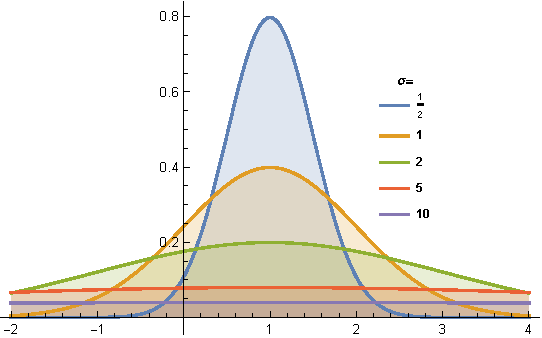
\includegraphics[width=0.8\columnwidth]{Normal.pdf}
\end{center}
\vspace{-1em}
\caption{\label{fig:pdfNorm}
PDF of Normal distributions with the same $\mu$ and different $\sigma$s.
}
\vspace{-1em}
\end{figure}


%defining torque
\begin{align} \nonumber
\tau &= \int_0^1\frac{1}{{\sigma \sqrt {2\pi } }}e^{{{ - \left( {x - \mu } \right)^2 } \mathord{\left/ {\vphantom {{ - \left( {x - \mu } \right)^2 } {2\sigma ^2 }}} \right. \kern-\nulldelimiterspace} {2\sigma ^2 }}} x \, dx\\ \nonumber
&= \frac{(-e^{-\frac{(-1+\mu)^2}{2\sigma^2}}+e^{-\frac{-\mu^2}{2\sigma^2}})\sigma}{\sqrt{2\pi}}\\ 
&+ \frac{1}{2}\mu(erf(\frac{1-\mu}{\sqrt{2}\sigma})+erf(\frac{\mu}{\sqrt{2}\sigma})) 
\end{align}
\begin{figure}
\begin{center}
	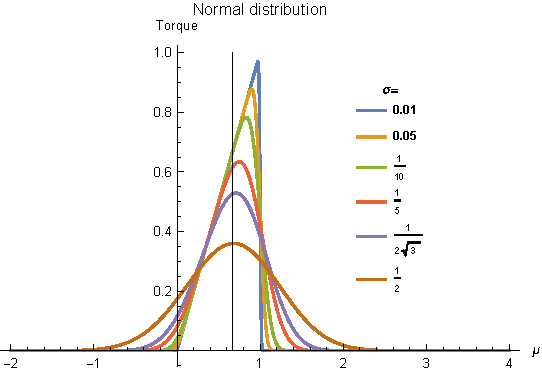
\includegraphics[width=0.8\columnwidth]{TorqueNormal.pdf}
\end{center}
\vspace{-1em}
\caption{\label{fig:torqueNorm}
Torque as a function of the mean position, $\mu$ which is the pushing location when the swarm is normally distributed with different standard deviations.
}
\vspace{-1em}
\end{figure}
%taking derivative of torque
\begin{align} 
\frac{d\tau}{d\mu} &= -\frac{e^{-\frac{{-1+\mu}^2}{2\sigma^2}}}{\sqrt{2\pi}\sigma} + \frac{1}{2}(erf(\frac{1-\mu}{\sqrt{2}\sigma})+erf(\frac{\mu}{\sqrt{2}\sigma})) 
\end{align}


%triangular distribution
\begin{align}
P(x)_{t} &=  \left\{
\begin{array}{ll}
    \frac{x-\mu + \sqrt{6} \sigma}{6\sigma^2}, &  \textrm{for   } \mu-\sqrt{6}\sigma \leq x \leq \mu\\
     \frac{-x+\mu + \sqrt{6} \sigma}{6\sigma^2}, &  \textrm{for   } \mu < x \leq \mu+ \sqrt{6}\sigma\\
     0, & \textrm{otherwise}\\
\end{array} 
\right.
\end{align}

\begin{figure}
\begin{center}
	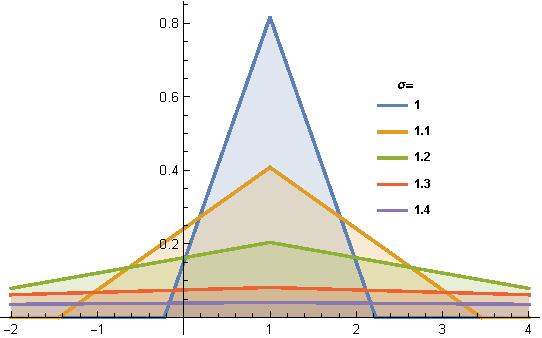
\includegraphics[width=0.8\columnwidth]{Triangular.pdf}
\end{center}
\vspace{-1em}
\caption{\label{fig:pdfTri}
PDF of Triangular distributions with the same $\mu$ and different $\sigma$s.
}
\vspace{-1em}
\end{figure}
%defining torque

\begin{strip}
\begin{align}
\tau_t &=  \left\{
\begin{array}{ll}
    \mu, &   \textrm{for     }\mu<1 \& \sqrt{6} \mu + 6 \sigma < \sqrt{6} \& \sqrt{6} \mu > 6 \sigma\\
    \frac{2-3\mu+3\sqrt{6}\sigma}{36\sigma^2}, & \textrm{for     } (\mu>1\&\sqrt{6}\mu \leq 6\sigma) | \mu =1 \& \sigma \geq \frac{1}{\sqrt{6}})\\
    \frac{-2+3\mu-2\mu^3+3\sqrt{6}\sigma}{36\sigma^2}, &   \textrm{for     } \mu<1 \& \sqrt{6}\mu+6\sigma\geq \sqrt{6} \& \sqrt{6} \mu \leq 6\sigma\\
    \frac{1}{2}-\frac{\sigma}{\sqrt{6}}, &   \textrm{for     } \mu = 1 \& \sigma < \frac{1}{\sqrt{6}}\\
    -\frac{2+\mu^3+3\sqrt{6}\mu^2\sigma+3\sqrt{6}\sigma(-1+2\sigma^2)-3\mu(1+6\sigma^2}{36\sigma^2} &  \textrm{for     } \mu<1 \& \sqrt{6} \mu + 6 \sigma \geq \sqrt{6} \& \sqrt{6} \mu > 6 \sigma\\
    \frac{2+\mu^3-3\sqrt{6}\mu^2\sigma+3\sqrt{6}\sigma(1-2\sigma^2)+3\mu(-1+6\sigma^2}{36\sigma^2} &  \textrm{for     } \mu>1 \& 0<\sqrt{6}\mu-6\sigma<\sqrt{6}\\
    \frac{1}{36}(18\mu-\frac{\mu^3}{\sigma^2} + \frac{3\sqrt{6}\mu^2}{\sigma}+6\sqrt{6}\sigma) &  \textrm{for     }  \sqrt{6} \mu+6\sigma<\sqrt{6}\&\sqrt{6}\mu\leq 6\sigma\\
     0, &  \textrm{otherwise}\\ 
\end{array} 
\right.
\end{align}
\end{strip}


\begin{figure}
\begin{center}
	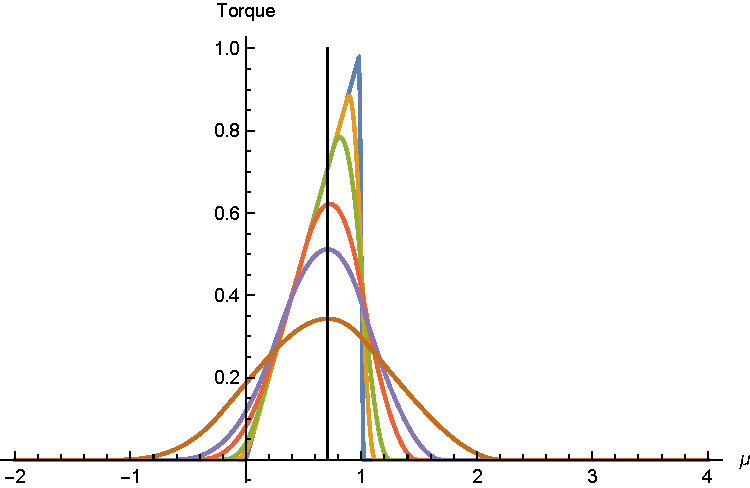
\includegraphics[width=0.8\columnwidth]{TorqueTri.pdf}
\end{center}
\vspace{-1em}
\caption{\label{fig:torqueTri}
Torque as a function of the mean position, $\mu$ which is the pushing location when the swarm is distributed by triangular distribution with different standard deviations.
}
\vspace{2em}
\end{figure}


\newpage
\begin{figure}
\begin{center}
	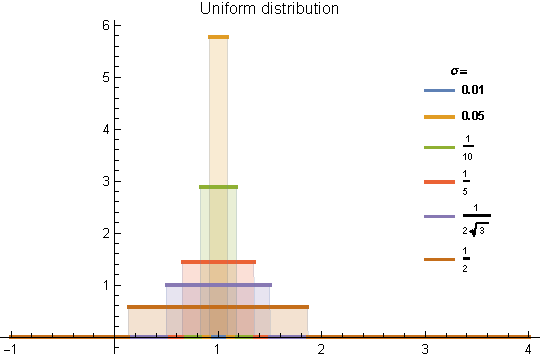
\includegraphics[width=0.8\columnwidth]{Uniform.pdf}
\end{center}
%\vspace{-1em}
\caption{\label{fig:pdfUni}
The Uniform distribution with different standard deviations and the same mean.
}
\vspace{-1em}
\end{figure}
%uniform torque
\begin{align}
\mu = \textrm{Max}[1-\sqrt{3}\sigma,\sqrt{3}\sigma]
\end{align}
\begin{figure}
\begin{center}
	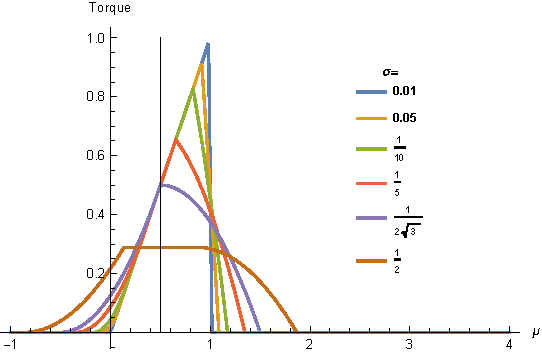
\includegraphics[width=0.8\columnwidth]{TorqueUni.pdf}
\end{center}
\vspace{-1em}
\caption{\label{fig:torqueUni}
Torque as a function of the mean position, $\mu$ which is the pushing location when the swarm is uniformly distributed with different standard deviations.
}
\vspace{-1em}
\end{figure}


\newpage

\section{Free object torque}
%torque normal free

\begin{strip}
\begin{align} \nonumber
\tau = \int_{-1}^1\frac{1}{{\sigma \sqrt {2\pi } }}e^{{{ - \left( {x - \mu } \right)^2 } \mathord{\left/ {\vphantom {{ - \left( {x - \mu } \right)^2 } {2\sigma ^2 }}} \right. \kern-\nulldelimiterspace} {2\sigma ^2 }}} x \, dx = \frac{(-e^{-\frac{(-1+\mu)^2}{2\sigma^2}}+e^{-\frac{-(1+\mu)^2}{2\sigma^2}})\sigma}{\sqrt{2\pi}}+ \frac{1}{2}\mu(erf(\frac{1-\mu}{\sqrt{2}\sigma})+erf(\frac{1+\mu}{\sqrt{2}\sigma})) 
\end{align}
\end{strip}
%torque triangular free


\begin{strip}
\begin{align}
\tau_t &=  \left\{
\begin{array}{ll}
    \mu, &   \textrm{for     }\sqrt{6}(1+\mu)\geq 6\sigma \& \sqrt{6}\mu + 6 \sigma < \sqrt{6} \& \sigma>0\\
     -\frac{1}{9\sigma^2},   & \textrm{for     } (\mu=-1\&3\sigma \geq \sqrt{6} | \mu <-1 \& \sqrt{6}\mu+6\sigma > \sqrt{6})\\
   \frac{1}{9\sigma^2}, & \textrm{for     } (\mu>1\&\sqrt{6}(1+\mu) \leq 6\sigma) | \mu =1 \& 3\sigma \geq \sqrt{6})\\
    -\frac{\mu(-3+\mu^2)}{18\sigma^2}, & -1<\mu<1 \& \sqrt{6}(1+\mu) <6\sigma \& \sqrt{6}\mu + 6\sigma\geq\sqrt{6}\\
    \frac{1}{2}-\frac{\sigma}{\sqrt{6}}, & \textrm{for     } \mu = 1 \& 0< \sigma < \sqrt{\frac{2}{\sqrt{3}}}\\
    -\frac{1}{2}+\frac{\sigma}{\sqrt{6}}, & \textrm{for     } \mu = -1 \&0< \sigma < \sqrt{\frac{2}{\sqrt{3}}}\\
    -\frac{2+\mu^3+3\sqrt{6}\mu^2\sigma+3\sqrt{6}\sigma(-1+2\sigma^2)-3\mu(1+6\sigma^2}{36\sigma^2} &  \textrm{for     }  \sqrt{6} \mu+6\sigma\geq\sqrt{6}\&\mu<1\&\sqrt{6}(1+\mu)\geq 6\sigma\\
   \frac{2+\mu^3-3\sqrt{6}\mu^2\sigma+3\sqrt{6}\sigma(1-2\sigma^2)+3\mu(-1+6\sigma^2}{36\sigma^2} &  \textrm{for     } \mu>1 \& -\sqrt{6}< \sqrt{6}\mu-6\sigma< \sqrt{6} \\
     \frac{2-\mu^3+3\sqrt{6}\mu^2\sigma+3\sqrt{6}\sigma(-1+2\sigma^2)+3\mu(1+6\sigma^2}{36\sigma^2} &  \textrm{for     } \mu>-1 \& -\sqrt{6}(1+\mu)<6\sigma\& \sqrt{6}\mu+6\sigma< \sqrt{6} \\
     \frac{-2+\mu^3+3\sqrt{6}\mu^2\sigma+3\sqrt{6}\sigma(-1+2\sigma^2)+3\mu(-1+6\sigma^2}{36\sigma^2} &  \textrm{for     } \mu<-1 \& -\sqrt{6}< \sqrt{6}\mu+6\sigma< \sqrt{6} \\
     0, &  \textrm{otherwise}\\
\end{array} 
\right.
\end{align}
\end{strip}


%torque uniform free




%pivoted comparisons:

\begin{figure}
\begin{center}
	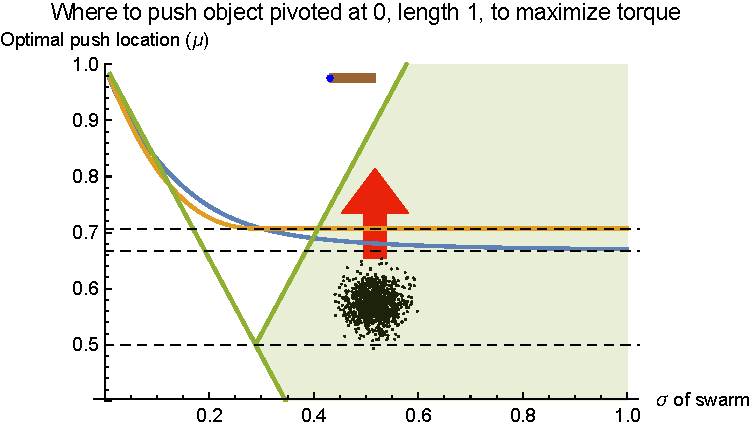
\includegraphics[width=0.8\columnwidth]{BestLocationPivot.pdf}
\end{center}
\vspace{-1em}
\caption{\label{fig:besLocPiv}
Comparison for three different distributions for the best location to push the object.
}
\vspace{0em}
\end{figure}


\begin{figure}
\begin{center}
	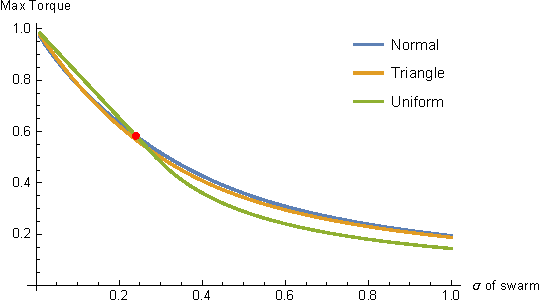
\includegraphics[width=0.8\columnwidth]{MaxTorquePivot.pdf}
\end{center}
%\vspace{0em}
\caption{\label{fig:maxTorPiv}
Comparison for three different distributions for the maximum torque possible.
}
\vspace{0em}
\end{figure}

%free comparisons

\begin{figure}
\begin{center}
	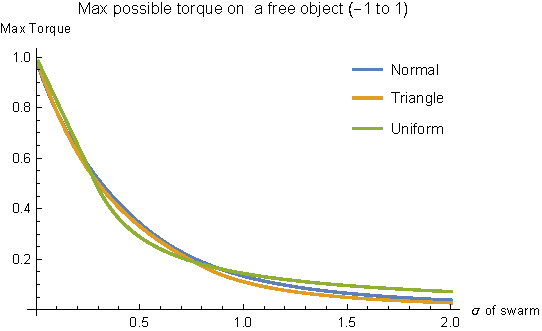
\includegraphics[width=0.8\columnwidth]{TorqueFreeComparison.pdf}
\end{center}
\vspace{-1em}
\caption{\label{fig:maxTorqueFree}
Comparison for three different distributions for the maximum torque possible.
}
\vspace{0em}
\end{figure}


\begin{figure}
\begin{center}
	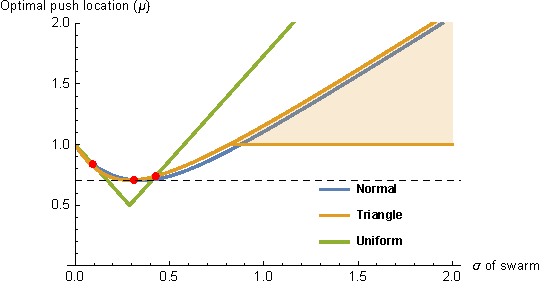
\includegraphics[width=0.8\columnwidth]{TorqueFreeBestPush.pdf}
\end{center}
%\vspace{0em}
\caption{\label{fig:bestLocFree}
Comparison for three different distributions for the best location to push the object.
}
\vspace{0em}
\end{figure}


